\documentclass[
  compress
  ,12pt
  %,draft
  %,handout % I don't see how this could ever work for my presentation!
]{beamer}

%%% Unknown packages
%\usepackage{beamerthemesplit}
%\usepackage{times}

% Provides script capital letters for math
\usepackage{mathrsfs}
%\usepackage{verbatim}

\newcommand{\bv}[1]{{\boldsymbol{#1}}}

%%% Fonts. Default font is computer modern
%\usefonttheme{default}
%\usefonttheme{professionalfonts} %allows you to use an external font w/o beamer replacements


%\usefonttheme[onlylarge]{serif}

%%  \usefonttheme[
%%    %onlysmall,
%%    onlylarge
%%    ] {structureitalicserif} %typesets structural text in italics with serifs

%% \usefonttheme[
%%   %onlysmall,
%%   onlylarge
%%   ] {structuresmallcapsserif} %Doesn't look too bad with onlylarge set

 \usefonttheme[
   % stillsansserifmath,
   % stillsansserifsmall,
   % stillsansseriftext,
   onlymath
 ]{serif} %onlymath option doesn't look too bad, eqns are more readable this way.


%%% Font families
%\usepackage{mathptmx} % not avail?
%\usepackage{helvet} % Helvetica is the standard sansserif font if you do not use the serif theme
%\usepackage{avant}   % fat, bubble-like sans serif letters
%\usepackage{chancery} % not available?
%\usepackage{utopia}  % not available?
%\usepackage{charter} % n/a
%\usepackage{times}

% A computer modern font available in T1 encoding.  As far as I
% can tell it doesn't look much different.
%\usepackage{lmodern}
%\usepackage[T1]{fontenc}



%%% Control the position of progress bars, titles, subtitles, etc. 
%\usetheme{default} % No navigation bars!
%\usetheme{boxes} % puts a box a in the head and footline, looks like default unless
                 % you also use \addheadbox and \addfootbox
%\usetheme{Bergen} % huge left-hand column. informal feel
%\usetheme{Boadilla} % shows page count at bottom.  requires institute
%\usetheme{Madrid} % Like Boadilla, but more color contrast
\usetheme{Pittsburgh} % right-flushed titles, otherwise very sparse
%\usetheme{Rochester}  % Huge title bars dominating the slide. square corners, no drop shadows
%\usetheme{Antibes}     % Large, Tree-based navigation at the top with sharp corners. Not bad
%\usetheme{JuanLesPins}  % Smooth version of Antibes, no lines in nav tree.
%\usetheme{Montpellier}  % To me, it looks like Antibes.  No box backgrounds.
%\usetheme{Darmstadt} %fuzzy top title bars, drop shadows, circle bullets,
                     % no side column. The top title is very busy
%\usetheme{Frankfurt}  % fuzzy title bars running across
                      % the top only, circular bullets, drop shadows,
                      % colored blocks with rounded corners, pretty nice
%\usetheme{Warsaw}  % Centrally divided top menu, no progress bullets, top
                   % of the screen is a bit busy but otherwise nice
%\usetheme{Berlin} % Square edges and bullets, no drop shadows, no rounded blocks
%\usetheme{Ilmenau} % Similar to Berlin, mini-nav frame, no drop shadows, rounded corners
%\usetheme{Dresden} % Like Berlin, but no block outlines. minimal context, lots of nav, but not bad

% \usetheme{Darmstadt} % Berlin with no bottom nav and rounded blocks, pretty nice, a bit too much at top though
%\usetheme{Frankfurt} % Very nice! Like Darmstadt but with less nav at the top (no 3rd bar)
                     % Still, if you don't use sections, there is an extra black bar at the top for no reason
%\usetheme{Singapore} % top title bar has a faded appearance, centered title names, minimal bullets.
%\usetheme{Szeged} % Lots of horizontal lines. Pretty nice but too cluttered at the top

% \usetheme{Berkeley} %side-bar menu screws up the spacing of slides somewhat, use with sidebartab
% \usecolortheme{sidebartab} % You really can't have long section names for this one

%\usetheme{Copenhagen} % tabular navigation, flat look (no shadows) too much top clutter
%\usetheme{Malmoe} % top cluttered
%\usetheme{Luebeck} % top cluttered
%\usetheme{Warsaw} % top is cluttered and even has a drop shadow


%\usetheme{Goettingen} % Looks like Berkely, but less obtrusive nav bar is on the right
                      % The right nav-bar cuts off your email address if you use it on the title page
\usecolortheme{sidebartab} % Used with sidebartab, it's really not bad

%\usetheme{Marburg} % A more dominant Goettingen, harder to read sidebar

%\usetheme{Hannover} % right flush titles, left-side nav, top looks a little empty

% This color theme works with all themes that show a table of contents in the sidebar.
\usecolortheme{sidebartab} 

%%% Color Themes: Make your colors bolder or more muted
%\usecolortheme{seahorse} % outer color theme, muted grey, a really nice one!, use with rose
                          % or lilly inner color themes
%\usecolortheme{rose}      % dark blue with relatively stark constrast levels
%\usecolortheme{lily}       % as above, but blocks do not have backround color
\usepackage{times}
\usepackage{units}

\setbeamercovered{invisible}
%\logo{
\includegraphics[width=.5in]{figures/word3}}
%\logo{FE Rodeo '07}
%\setbeamercolor{title}{fg=red!80!black,bg=red!20!white}

\title{Double-Diffusive Convection in Porous Media}
\author{J.~W.~Peterson\inst{1}
  \and B.~T.~Murray\inst{2}
  \and G.~F.~Carey\inst{3}
}


\date[FEF 2007]{March 26--28, 2007}


%\institute[UT-Austin]{Univ.\ of Texas at Austin}
\institute[University of Texas and SUNY]{
  \inst{1}Dept.\ of Aerospace Engineering\\
     UT-Austin
  \and
  \inst{2}Professor, Dept.\ of Mechanical Engineering\\
  SUNY Binghamton
  \and
  \inst{3}Professor, Inst.\ for Comp.\ and Engineering Science\\
  UT-Austin
}


%\AtBeginSection[]{\frame{\tableofcontents[current]}}

\setbeamercovered{transparent}


\newcommand{\D} [2]{\frac{\partial #1}{\partial #2}}
\newcommand{\KT}{\mbox{$\kappa_{T}$}}
\newcommand{\KS}{\mbox{$\kappa_{S}$}}

\begin{document}


  
\begin{frame}
  \titlepage
\end{frame}


\begin{frame}
  \frametitle{Physical Model}
      \begin{itemize}
      \item{``Double'' diffusion $\Rightarrow$ both heat and chemical (solute) species are diffusing}
      \item{Heat and solute have competing affects on background fluid density}
      \item{Ex: Heated Salt Water
	\begin{itemize}
	\item{Warm water is slightly less dense (rises)}
	\item{Salty water is slightly more dense (falls)}
	\item{Natural convection ``cells'' can develop }
	\end{itemize}
      }
      \end{itemize}
\end{frame}

\begin{frame}[t]
  \frametitle{Governing Equations}
  \begin{eqnarray}
    \label{eqn:p_strong}
    \nabla \cdot \alert<2>{\bv{b}} - \nabla^2 p &=& 0 \\
    \label{eqn:T_strong}
    \D{T}{t} + \left( \alert<2>{\bv{b}}-\nabla p\right) \cdot \nabla T - \nabla^2{T} &=&0 \\
    \label{eqn:S_strong}
    \frac{\phi}{\sigma} \D{S}{t} +
    \left( \alert<2>{\bv{b}}-\nabla p\right) \cdot \nabla S -  \alert<3>{\kappa} \nabla^2{S}&=&0 
  \end{eqnarray}

  \only<2>
  {
    \begin{equation}
      \nonumber
      \bv{b} = ( \kappa R_S S - R_T T ) \hat{e}_{g}
    \end{equation}
  }

  \only<3>
  {
    \begin{eqnarray}
      \nonumber
      \kappa &=& \frac{\text{Solute Diffusivity}}{\text{Thermal Diffusivity}} \ll 1 \\
      \nonumber
      &=& Le^{-1}
    \end{eqnarray}
  }
\end{frame}


%% \begin{frame}[t]
%%   \frametitle{Stabilization}
%%   \begin{itemize}
%%   \item<1->
%%     {
%%       For small $\kappa$ on coarse grids, the Galerkin method is known to perform poorly.
%%     }
%%   \item<2->
%%     {
%%       We add an additional stabilizing term:
%%     }
%%   \end{itemize}
%%   \visible<1->
%%   {
%%     \begin{equation}
%%       \nonumber
%%       \int_{\Omega} \left(  \frac{\phi}{\sigma}\frac{\partial S^h}{\partial t} +
%%       \left( \bv{b}^h -\nabla p^h \right) \cdot \nabla S^h  \right) v^h
%%       + \kappa \nabla S^h \cdot \nabla v^h \;dx
%%       \end{equation}
%%       \visible<2->
%%       {
%% 	\begin{equation}
%% 	  \small
%%       \nonumber
%%       + \underbrace{\int_{\Omega'} \tau \left( \left(\bv{b}^h - \nabla p^h\right) \cdot \nabla v^h \right) \left[
%% 	\frac{\phi}{\sigma} \D{S^h}{t} +
%% 	\left( \bv{b}^h-\nabla p^h\right) \cdot \nabla S^h - \kappa \nabla^2 S^h \right]dx
%%       }_{\text{Stabilization Term}}
%%       \end{equation}
%%       }
%%       \begin{equation}
%%       \nonumber
%%       %\label{eqn:S_stabilized}
%%       =\int_{\partial \Omega} \kappa \left( \nabla S \cdot \hat{n} \right) v^h \; ds
%%     \end{equation}
%%   }
%% \end{frame}

\begin{frame}
  \frametitle{Solute and Temperature Contours}
  \vspace{-.25in}
  \begin{center}
    \begin{tabular}{cc} \\
      %\includegraphics[viewport=80 105 580 665,clip=true,angle=-90,width=0.45\textwidth]{figures/s_150x150_kappa_0_03}&
      %\includegraphics[viewport=80 105 580 665,clip=true,angle=-90,width=0.45\textwidth]{figures/t_150x150_kappa_0_03}\\
    \includegraphics[viewport=80 105 580 665,clip=true,angle=-90,width=0.45\textwidth]%
		    {figures/s_150x150_kappa_0_03_PRESENTATION}&
    \includegraphics[viewport=80 105 580 665,clip=true,angle=-90,width=0.45\textwidth]%
		    {figures/t_150x150_kappa_0_03_PRESENTATION}\\
    Solute Contours & Temperature Contours
    \end{tabular}
  \end{center}
\end{frame}

%% \begin{frame}
%%   \frametitle{Representative Adapted Grid}
%%   \vspace{-.25in}
%%   \begin{center}
%%       \includegraphics[viewport=80 105 580 665,clip=true,angle=-90,width=0.75\textwidth]{figures/grid_adaptive_kappa_0_03}
%%   \end{center}
%% \end{frame}

\begin{frame}[t]
  \frametitle{Sherwood Number}
  \begin{itemize}
  \item {The total solute (or heat) flux to a wall is an important engineering quantity of interest.}
  \item {The Sherwood number is defined as:
    \begin{equation}
      \nonumber
      N_S := -\int_{\partial \Omega_D} \!\!\!\!\!\!\! \nabla S \cdot n \;dx 
    \end{equation}
    }
  \item{For large $R_T, Le,$ it is known that 
    \begin{equation}
      \nonumber
      N_S \approx \sqrt{R_T Le} = \sqrt{\frac{R_T}{\kappa}}
    \end{equation}
  }
  \end{itemize}
\end{frame}




\begin{frame}
  \frametitle{Sherwood Number Computations}
  \vspace{-.25in}
  \begin{center}
      \includegraphics[viewport=10 10 560 725 ,clip=true,angle=-90,width=0.8\textwidth]{figures/Nu_vs_Le}
  \end{center}
\end{frame}





%%%%%%%%%%%%%%%%%%%%%%%%%%%%%%%%%%%%%%%%%%%%%%%%%%%%%%%%%%%%%%%%%%%%%%%%%%%%%%%%%%%%%%%%%%%%%%%%%%%%
%\section{Boundary Flux Integrals}

\begin{frame}
      \begin{itemize}
      \item{
	The problem of determining the Sherwood number can be thought of generically.}

      \item{
	We consider the integrated flux $I$ of some variable $u$ through
	a boundary $\Gamma \subseteq \partial \Omega$

	\begin{equation}
	  \nonumber
	  I := \int_{\Gamma} k \nabla u \cdot n \;ds = -\int_{\Gamma} \sigma \cdot n \;ds 
	\end{equation}
      }
        
      \item{For example, $I$ could be total mass/thermal flux, Lift, Drag, etc.}

      \item{Differentiating the FE solution
	%to obtain $\sigma\cdot n$ is only
	%$\mathcal{O}(h^p)$ accurate.
	generally yields 
	\begin{equation}
	  \nonumber
	  \| \sigma - \sigma_h \|_{L_2(\Gamma)} \approx \mathcal{O}(h^p)
	\end{equation}
      } 
	
      \end{itemize}
\end{frame}


\begin{frame}
  \frametitle{S.~C.~Boundary Flux Literature}
      \begin{itemize}
      \item
	{
          Many schemes for computing superconvergent boundary fluxes have been investigated:

	  \begin{itemize}
	  \item{J.~Douglas, T.~Dupont, and M.~Wheeler (1974)}
	  \item{M.~Wheeler (1979)}
	  \item{Carey et al. (1982, 2002)}
	  \item{Hughes, Larson, Cochburn, Wahlbin, Babu{\v{s}}ka, \ldots}
	  \end{itemize}
	}
	
      \item{Under some restrictions
	\begin{equation}
	  \nonumber
	  \| \sigma - \sigma_h \|_{L_2(\Gamma)} \approx \mathcal{O}(h^{p+1})
	\end{equation}

	is generally possible, see e.g.\ Douglas.}
	
      \end{itemize}
\end{frame}


\begin{frame}
  \frametitle{Model Problem: Poisson}
	\begin{equation}
	  \nonumber
	  -\nabla \cdot \left( k \nabla u \right)=f
	\end{equation}
      \begin{itemize}
      \item<1->{For all $\phi_i \neq 0$ on $\partial \Omega$
      \begin{equation}
	\nonumber
	-\int_{\partial \Omega} \left( \sigma\only<2->{\alert<2>{_h}} \cdot n\right)\phi_i \;ds =
	\int_{\Omega} k\nabla u\only<2->{\alert<2>{_h}} \cdot \nabla \phi_i - f\phi_i \;dx 
	\end{equation}

      }
	
      \item<3->{Can use this relation to solve for improved flux approximation.}

      \item<4->{Difficulties \ldots
	\begin{itemize}
	  \item {$\sigma \cdot n$ discontinuous at a node}
	  \item {$n$ not well-defined at nodes}
	  \item {3D extension}
	\end{itemize}
      }
      \end{itemize}
\end{frame}




\begin{frame}
      \begin{itemize}
      \item{
        It's simpler if we don't care about pointwise values of $\sigma \cdot n$,
	i.e.\ only the integrated flux is
	important.}

      \item{Carey (2002) uses partition of unity method: on $\partial \Omega$,
	\begin{equation}
	  \nonumber
	  \sum_{i=1}^N \phi_i = 1
	\end{equation}
	where $N$ is the number of nodes on $\partial \Omega$, to show that
	\begin{eqnarray}
	  \nonumber
	  -\int_{\partial \Omega} \left(\sigma_h \cdot n\right)
	   \underbrace{\left(\sum_{i=1}^N \phi_i \right)}_{=1} ds &=&
	\sum_{i=1}^N \int_{\Omega} k\nabla u_h \cdot \nabla \phi_i - f\phi_i \;dx
	%\\
	%I &=& \sum_{i=1}^N \int_{\Omega} k\nabla u_h \cdot \nabla \phi_i - f\phi_i \;dx 
	\end{eqnarray}
      }
      \end{itemize}
\end{frame}




\begin{frame}
      \begin{itemize}
      \item{
        We can do something similar on $\Gamma \subset \partial \Omega$: let $S$ be the set of elements
	which have a node on $\Gamma$, and let
	\begin{equation}
	  \nonumber
	  \sum_{i=1}^M \phi_i = 1 
	\end{equation}
	on $\Gamma$ where $M$ is the number of nodes on $\Gamma$.
	%, and $\Gamma_{+}$ is a slightly
	%larger domain.
      }
	
      \item{
	Then we have
	\begin{eqnarray}
	  \nonumber
	  \sum_{i=1}^M \int_{\Gamma_{+}}-\left(\sigma_h\cdot n\right)  \phi_i \;ds =
	  \sum_{i=1}^M \int_{S} k\nabla u_h \cdot \nabla \phi_i - f\phi_i \;dx 
	\end{eqnarray}
      }
      \end{itemize}
\end{frame}


\begin{frame}
  \begin{center}
    \includegraphics[width=.4\textwidth,angle=-90]{figures/square}    
  \end{center}

      \begin{itemize}
      \item{
        Example: $\Gamma$ is the bottom side, $\Gamma_{+}$ extends into the first element
	of the two adjacent sides.
	}
      \end{itemize}
\end{frame}





\begin{frame}
      \begin{itemize}
      \item{We can rewrite this as, let $ q_h  := -\left(\sigma_h \cdot n\right)$
	\begin{eqnarray}
	  \nonumber
	  \sum_{i=1}^M \int_{\Gamma} q_h \phi_i ds +
	  \int_{\Gamma_{+} \setminus \Gamma} \!\!\!\!\!\!\! q_h \phi_1 ds +
	  \int_{\Gamma_{+} \setminus \Gamma} \!\!\!\!\!\!\! q_h \phi_M ds 
	  &=&\\
	  \nonumber
	  \sum_{i=1}^M \int_{S} k\nabla u_h \cdot \nabla \phi_i - f\phi_i \;dx 
	\end{eqnarray}
	or,
	\begin{eqnarray}
	  \nonumber
	  I_h  &=&
	  \sum_{i=1}^M \int_{S} k\nabla u_h \cdot \nabla \phi_i - f\phi_i \;dx -
	  \int_{\Gamma_{+} \setminus \Gamma} \!\!\!\!\!\!\! q_h \phi_1 ds -
	  \int_{\Gamma_{+} \setminus \Gamma} \!\!\!\!\!\!\! q_h \phi_M ds 
	\end{eqnarray}
	}

      \item{If $\Gamma_{+} \setminus \Gamma$ is a Neumann boundary, the extra terms on the r.h.s.\
	are known.  In general the extra terms aren't known.}
      \end{itemize}
\end{frame}


\begin{frame}[t]
      \only<1>
	  {
	    \begin{center}
	      \includegraphics[width=.4\textwidth,angle=-90]{figures/nub_picture_mesh_only}
	    \end{center}
	      \begin{itemize}
	      \item {Another illustration using quadratic
		elements: $\Gamma$ is the piece of the boundary shown.}
	      \end{itemize}
	  }

      \only<2>
	  {
	    \begin{center}
	      \includegraphics[width=.4\textwidth,angle=-90]{figures/nub_picture_green_only}
	    \end{center}
	      \begin{itemize}
	      \item {Basis functions which sum to 1 on $\Gamma$.}
	      \end{itemize}
	  }
	  
      \only<3>
	  {
	    \begin{center}
	      \includegraphics[width=.4\textwidth,angle=-90]{figures/nub_picture_all}
	    \end{center}
	      \begin{itemize}
	      \item {``Extra'' support of the first and last basis functions which create $\Gamma_{+}$.}
	      \end{itemize}
	  }

\end{frame}





%% \begin{frame}
%%       \begin{itemize}
%%       \item{We can approximate the extra
%% 	terms using the ``classical'' $\mathcal{O}(h^p)$
%% 	technique of differentiating the 
%% 	FE solution.
%%       }
	
%%       \item{Is this still a more accurate result?}
	
%%       \end{itemize}
%% \end{frame}







%\begin{frame}
  \frametitle{Test Problem}
  \begin{equation}
    \nonumber
    -\Delta u = f \in \Omega
  \end{equation}
  \begin{itemize}
  \item{$\Omega$ = unit square}
  \item{Dirichlet data and $f$ are chosen so that the exact solution is $u=\frac{12}{(1+x+y)^2}$.}
  \item{$\Gamma$ is chosen as the bottom face of the square.}
  \item{The exact solution is $I=9$.}
  %\item{$\sigma$ is not a polynomial.}
  \item{$\sigma \cdot n$ is discontinuous at the corners.}
  \end{itemize}
\end{frame}

\begin{frame}
  \frametitle{Bilinear Elements}
  \vspace{-.25in}
  \begin{center}
    \includegraphics[width=\textwidth]{figures/dcf_bilinear_presentation}    
  \end{center}
\end{frame}

\begin{frame}
  \frametitle{Biquadratic Elements}
  \vspace{-.25in}
  \begin{center}
    \includegraphics[width=\textwidth]{figures/dcf_biquadratic_presentation}    
  \end{center}
\end{frame}



\begin{frame}[t]
  \frametitle{Time-Dependent Problems}
  \begin{itemize}
%%     \item{The extension to time-dependent
%%       %systems of
%%       equations is straightforward.}
    \item{Consider a $\theta$-scheme for:}
  \end{itemize}
%%   \only<1>
%%   {
%%   \begin{equation}
%%     \nonumber
%%     \frac{\partial \bv{U}}{\partial t} = f(\bv{U})
%%   \end{equation}
%%   }
%%   \only<2>
%%   {
%%   \begin{equation}
%%     \nonumber
%%     \left(\frac{\partial \bv{U}}{\partial t},v\right)_{\Omega} =
%%     \left(f\left(\bv{U}\right), v\right)_{\Omega} +
%%     \left( \right)_{\partial \Omega}
%%   \end{equation}
%%   }

  \begin{equation}
    \nonumber
    \frac{\partial u}{\partial t} = \nabla \cdot \left(k \nabla u\right) + f
  \end{equation}

  \only<2>
  {
  \begin{eqnarray}
    \nonumber
    \int_{\Omega} \alert{\frac{\partial u}{\partial t}} \phi_i \;dx &=&
    \int_{\Omega} \left(-k \nabla u \cdot \nabla \phi_i +f\phi_i\right) dx
    \\
    \nonumber
    &+&
    \int_{\partial \Omega} \left( k\nabla u \cdot n\right)\phi_i \;ds
  \end{eqnarray}
  }

  \only<3>
  {
  \begin{eqnarray}
    \nonumber
    \alert<3>{\frac{1}{\Delta t}}\int_{\Omega} \left(\alert<3>{u^{n+1} - u^n}\right) \phi_i \;dx &=&
    \int_{\Omega} \left(-k \nabla u_{\alert<3>{\theta}} \cdot \nabla \phi_i +f\phi_i\right)dx
    \\
    \nonumber
    &-&
%    \only<5>{\underbrace{ }
      \int_{\partial \Omega} \left( \sigma_{\alert<3>{\theta}} \cdot n\right)\phi_i \;ds
%      \only<5>{}_{hi}}
  \end{eqnarray}
  }
  
  \only<4>
  {
  \begin{eqnarray}
    \nonumber
    \alert<3>{\frac{1}{\Delta t}}\int_{\Omega} \left(\alert<3>{u^{n+1} - u^n}\right) \phi_i \;dx &=&
    \underbrace{ 
    \int_{\Omega} \left(-k \nabla u_{\alert<3>{\theta}} \cdot \nabla \phi_i +f\phi_i\right)dx
    }_{\alert{\text{To LHS}}}
    \\
    \nonumber
    &-&
    %\underbrace{ 
      \int_{\partial \Omega} \left( \sigma_{\alert<3>{\theta}} \cdot n\right)\phi_i \;ds
    %}_{\alert{\text{To LHS}}}
  \end{eqnarray}
  }

  \only<5>
  {
  \begin{eqnarray}
    \nonumber
    -\int_{\partial \Omega} \left( \sigma_{\theta} \cdot n\right) \phi_i \;ds &=&
    \frac{1}{\Delta t}\int_{\Omega} \left(u^{n+1} - u^n\right) \phi_i \;dx
    \\
    \nonumber
    &+&
    \int_{\Omega} \left(k \nabla u_{\theta} \cdot \nabla \phi_i -f\phi_i \right)dx 
  \end{eqnarray}

  \begin{itemize}
    \item {The formula allows us to recover the flux at any point $t_{\theta}$ in the interval.}
  \end{itemize}
  }
\end{frame}



\begin{frame}
  \frametitle{Double-Diffusive Convection}
  \begin{itemize}
    \item{ We now proceed to use the flux formula to
      compute Sherwood numbers for the double-diffusion problem
      \vspace{-.2in}
      \begin{center}
	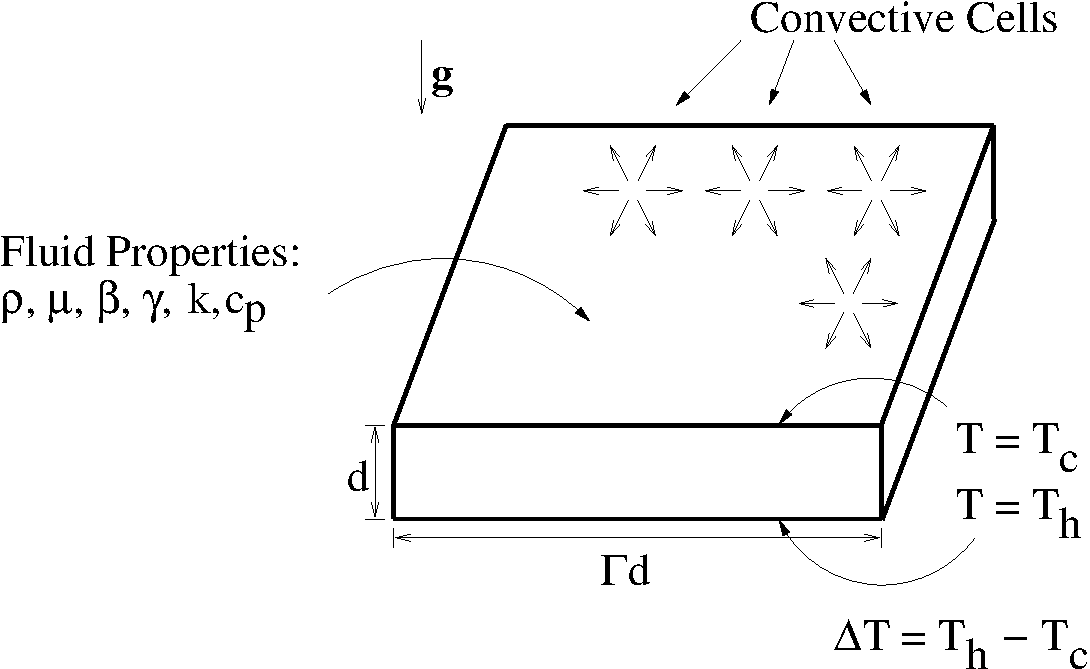
\includegraphics[width=.3\textwidth,angle=-90]{figures/setup}
      \end{center}
    }
    \item{The goal is to compute the steady state value of 
      $I := -\int\nabla S \cdot n \;dx$ or $-\int\nabla T \cdot n \;dx$
      at the bottom (or top) of the enclosure.}
  \end{itemize}
\end{frame}



\begin{frame}
  \frametitle{Double-Diffusive Convection}
  \begin{itemize}
    \item{As a simple test problem, we consider the case $\kappa=1$.}
    \item{In this case, $T=S$ at steady state so it suffices to consider
      the flux of only a single variable. }
  \end{itemize}
\end{frame}

\begin{frame}
  \frametitle{Double-Diffusive Convection}
    \vspace{-.25in}
    \begin{center}
	\includegraphics[width=.8\textwidth]{figures/kappa1_solute_error_bilinears.pdf}    
  \end{center}
    \vspace{-.2in}
    \begin{itemize}
      \item{Surprisingly, the classical method is actually \emph{better} here.}
    \end{itemize}
\end{frame}

\begin{frame}
  \frametitle{Double-Diffusive Convection}\vspace{-.25in}
    \begin{center}
	\includegraphics[width=.8\textwidth]{figures/kappa1_solute_error_biquadratics.pdf}    
  \end{center}
\vspace{-.2in}
    \begin{itemize}
      \item{For biquadratics, the boundary flux formula recovers the $p+1$ rate.}
    \end{itemize}
\end{frame}





\begin{frame}
  \frametitle{$h$-Adaptivity}
  \begin{itemize}
    \item{We now employ an extremely simple flux jump error estimator to drive adaptivity
  \begin{equation}
    \nonumber
    \eta^{\text{FLUX}}_K := \left( {h_K} \int_{\partial K} |R_K|^2 ds \right)^{1/2}
    \label{eqn:flux_indicator}
  \end{equation}
  }

    \item{
where $R_K$ is the local residual defined by
\begin{equation}
  \nonumber
  R_K := \left\{
    \begin{array}{cl}
      0, & s \in \partial K \cap \Gamma_D \\
      g_N - \nabla u_h \cdot n_K, & s \in \partial K \cap \Gamma_N \\
      \frac{1}{2}(\nabla u_h|_L - \nabla u_h|_K) \cdot n_K, & s \in \partial K \cap \partial L \neq \emptyset
    \end{array}
    \right.
  \label{eqn:residual}
\end{equation}
%% where $g_N$ is given Neumann boundary data, $n_K$ is the outward unit
%% normal for cell $K$, and cell $L$ shares an edge (face) with cell $K$
%% in the finite element mesh.
}
  \end{itemize}
\end{frame}

\begin{frame}
  \frametitle{Bilinear Adaptivity}
  \begin{center}
	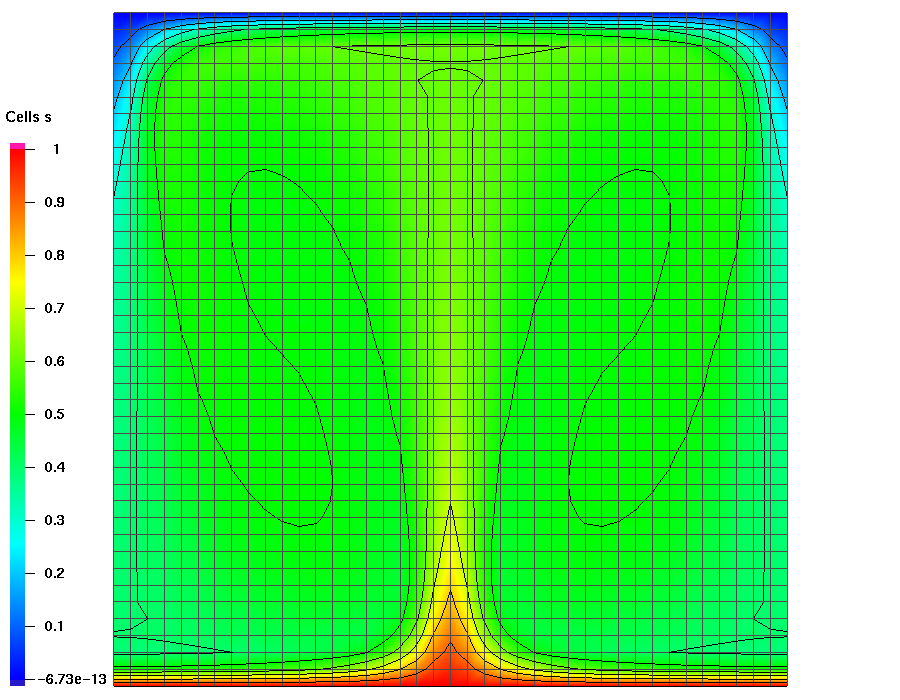
\includegraphics[width=.8\textwidth]{figures/bilinear_amr_0000}    
  \end{center}
\end{frame}
  
\begin{frame}
  \frametitle{Bilinear Adaptivity}
  \begin{center}
	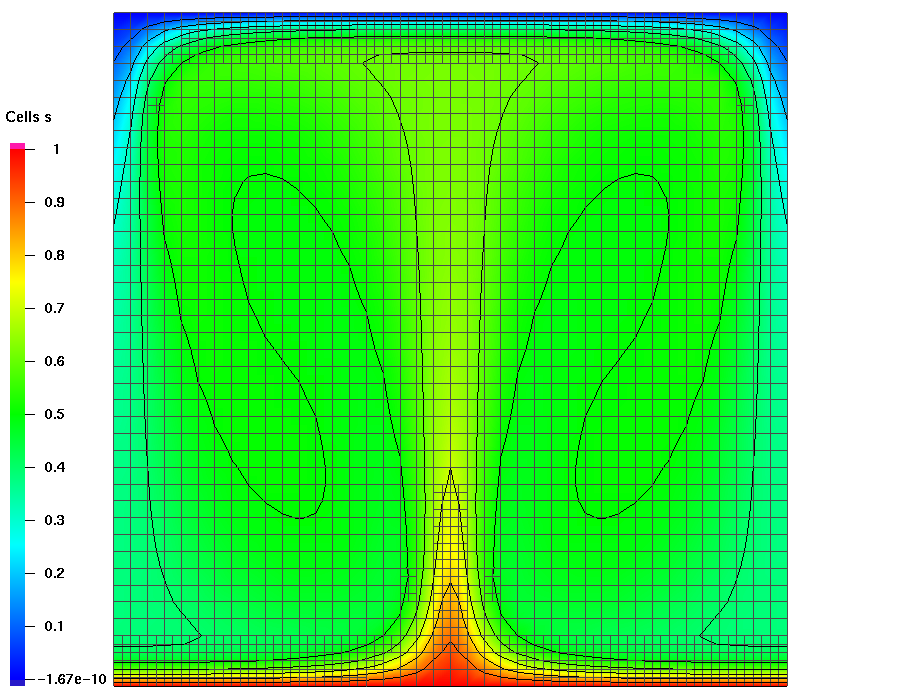
\includegraphics[width=.8\textwidth]{figures/bilinear_amr_0001}    
  \end{center}
\end{frame}

  \begin{frame}
  \frametitle{Bilinear Adaptivity}
  \begin{center}
	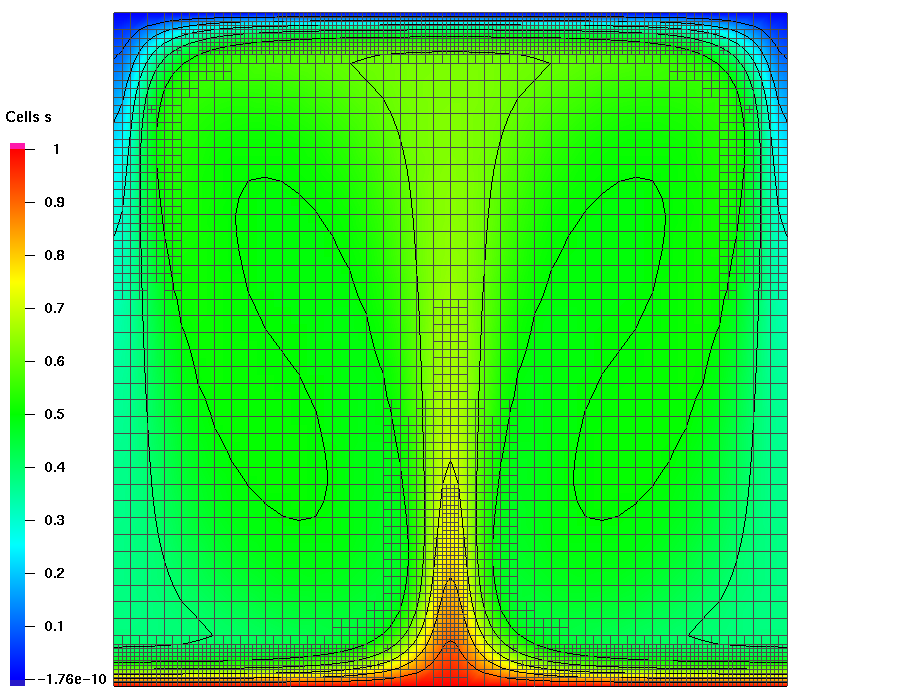
\includegraphics[width=.8\textwidth]{figures/bilinear_amr_0002}    
  \end{center}
\end{frame}
\begin{frame}
  \frametitle{Bilinear Adaptivity}
  \begin{center}
	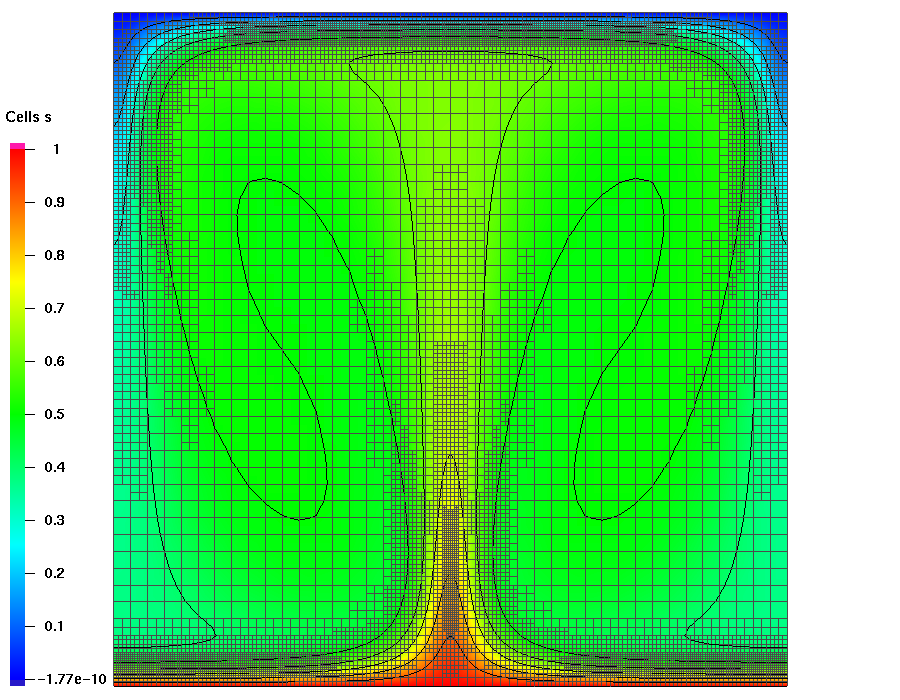
\includegraphics[width=.8\textwidth]{figures/bilinear_amr_0003}    
  \end{center}
\end{frame}
\begin{frame}
  \frametitle{Bilinear Adaptivity}
  \begin{center}
	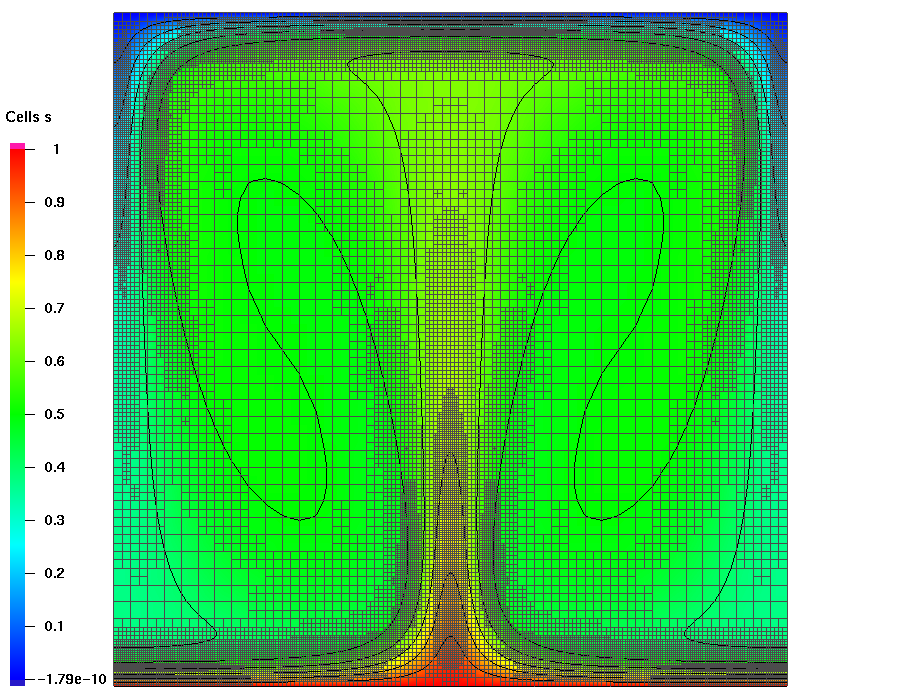
\includegraphics[width=.8\textwidth]{figures/bilinear_amr_0004}    
  \end{center}
\end{frame}
\begin{frame}
  \frametitle{Bilinear Adaptivity}
  \begin{center}
	\includegraphics[width=.9\textwidth]{figures/bilinear_adapt_vs_unif_thermal}    
  \end{center}
\end{frame}
\begin{frame}
  \frametitle{Bilinear Adaptivity}
  \begin{center}
	\includegraphics[width=.9\textwidth]{figures/bilinear_adapt_vs_unif_solute}    
  \end{center}
\end{frame}





%%   }
%%   \only<2>
%%       {
%% 	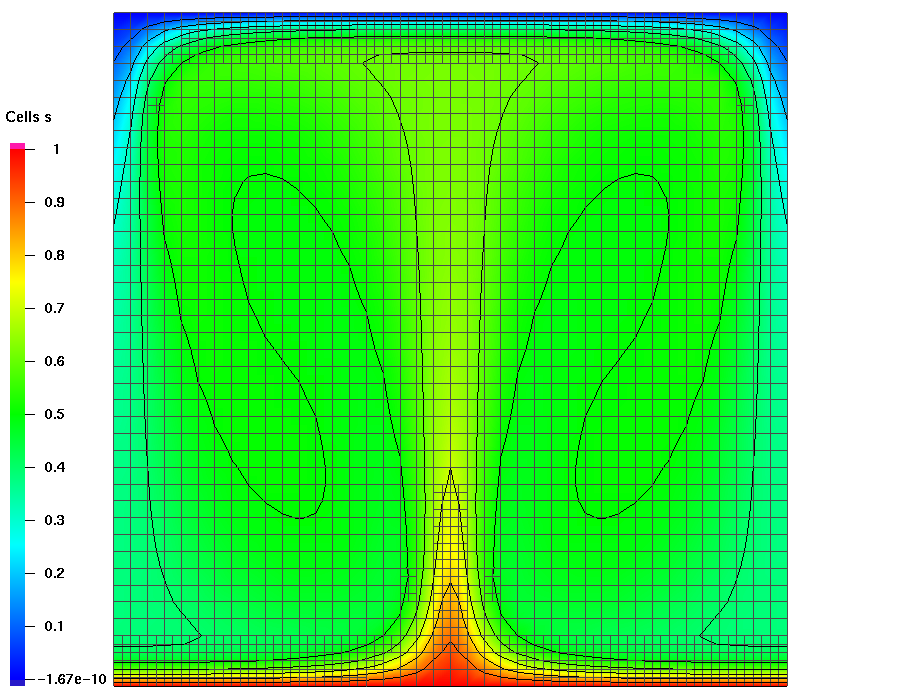
\includegraphics[width=.8\textwidth]{figures/bilinear_amr_0001}    
%%       }
%%   \only<3>
%%       {
%% 	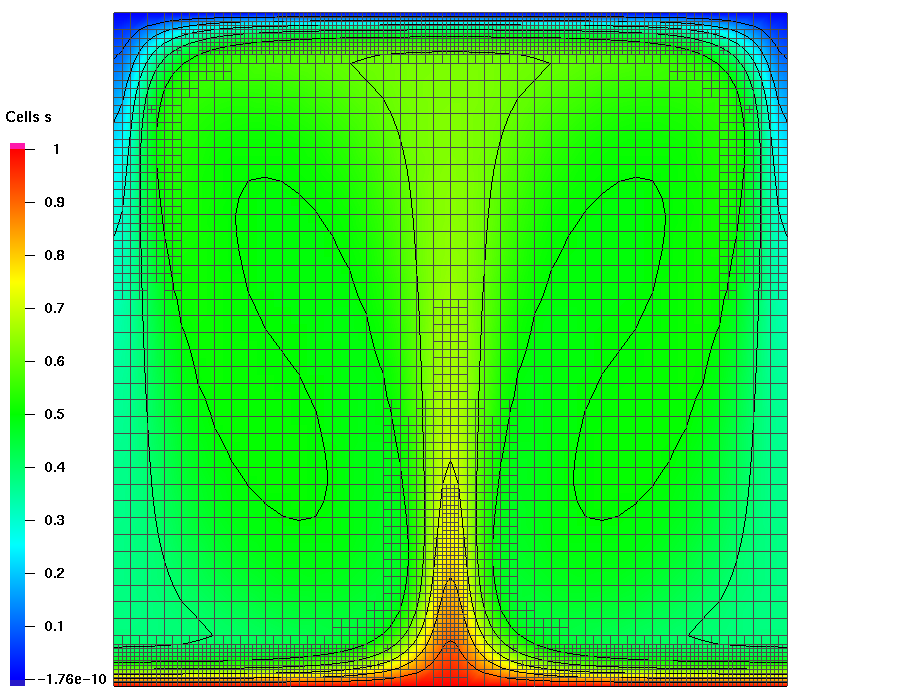
\includegraphics[width=.8\textwidth]{figures/bilinear_amr_0002}    
%%       }
%%   \only<4>
%%       {
%% 	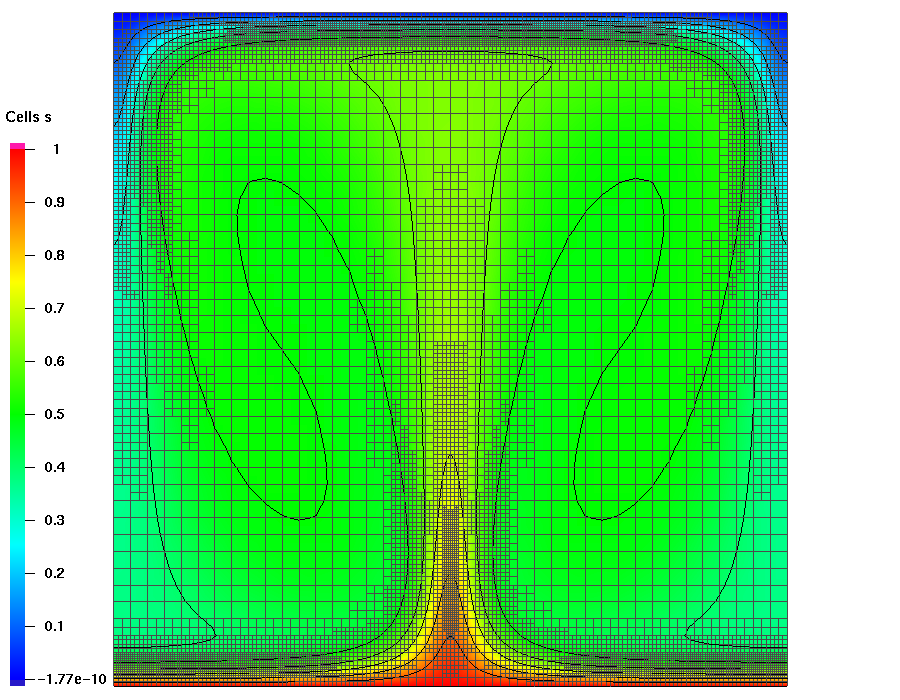
\includegraphics[width=.8\textwidth]{figures/bilinear_amr_0003}    
%%       }
%%   \only<5>
%%       {
%% 	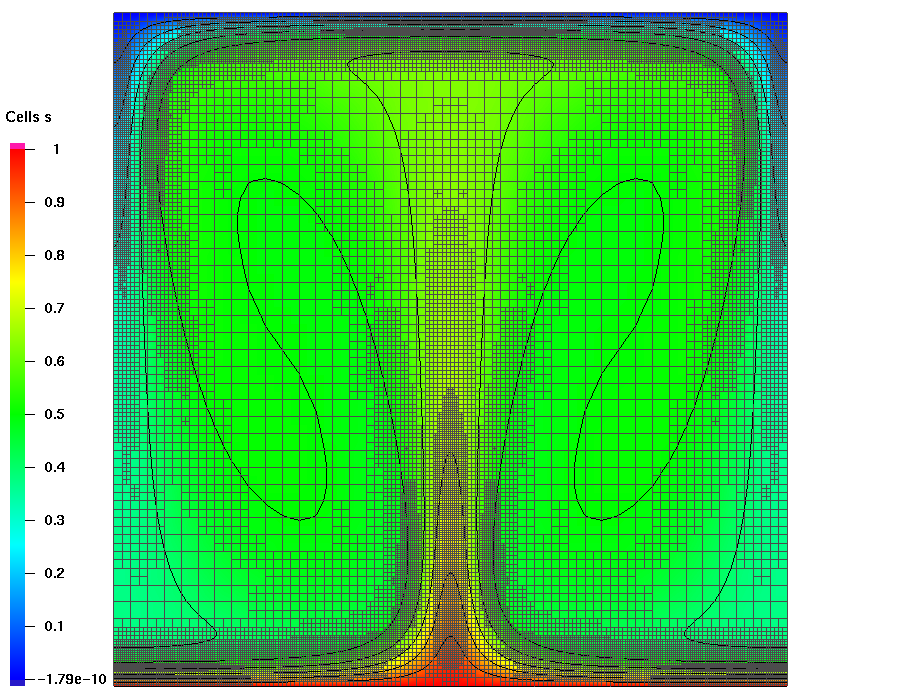
\includegraphics[width=.8\textwidth]{figures/bilinear_amr_0004}    
%%       }
%%   \only<6>
%%       {
%% 	\includegraphics[width=.8\textwidth]{figures/bilinear_adapt_vs_unif_thermal}    
%%       }
%%   \only<7>
%%       {
%% 	\includegraphics[width=.8\textwidth]{figures/bilinear_adapt_vs_unif_thermal}    
%%       }
%%   \end{center}
      

\begin{frame}
  \frametitle{Biquadratic Adaptivity}
  \begin{center}
	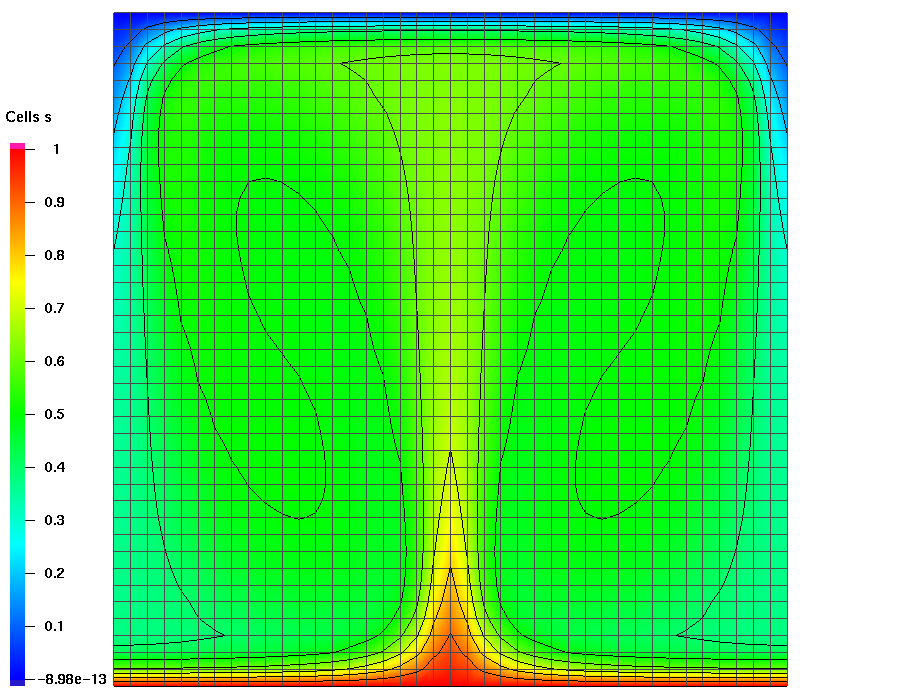
\includegraphics[width=.8\textwidth]{figures/biquad_amr_0000}    
  \end{center}
\end{frame}
  
\begin{frame}
  \frametitle{Biquadratic Adaptivity}
  \begin{center}
	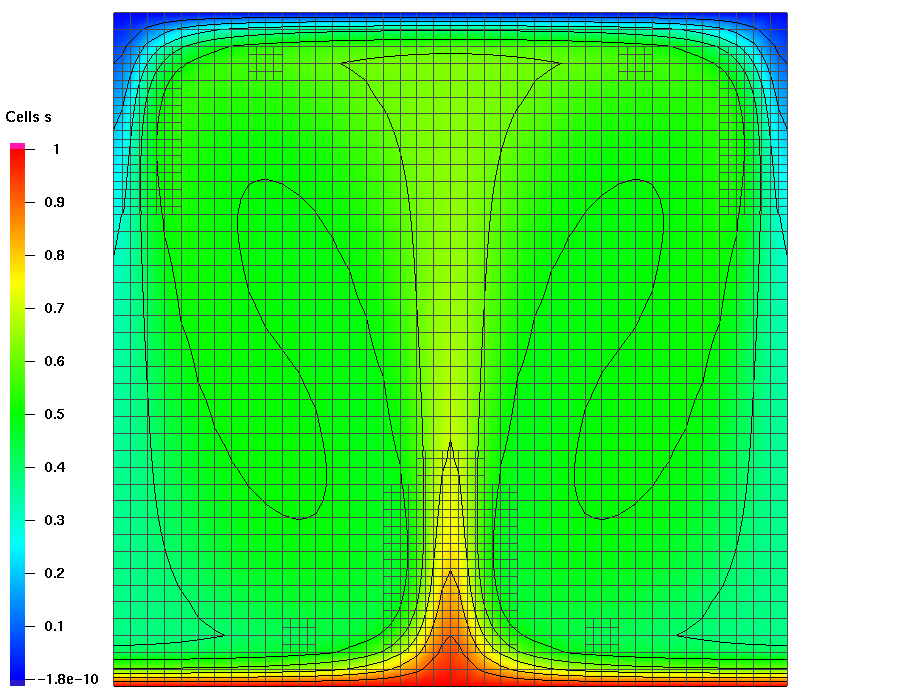
\includegraphics[width=.8\textwidth]{figures/biquad_amr_0001}    
  \end{center}
\end{frame}

  \begin{frame}
  \frametitle{Biquadratic Adaptivity}
  \begin{center}
	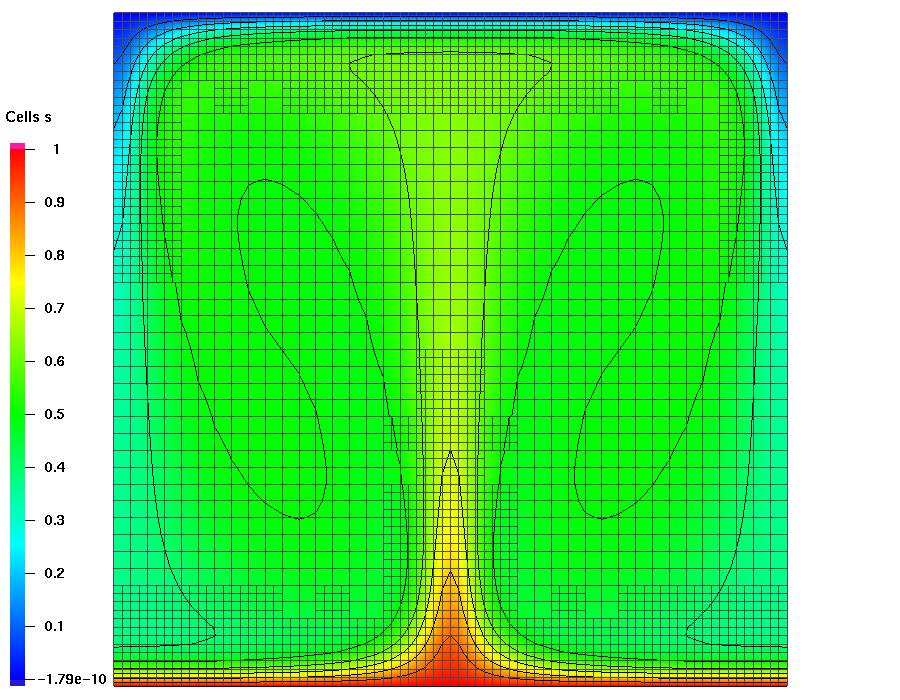
\includegraphics[width=.8\textwidth]{figures/biquad_amr_0002}    
  \end{center}
\end{frame}
\begin{frame}
  \frametitle{Biquadratic Adaptivity}
  \begin{center}
	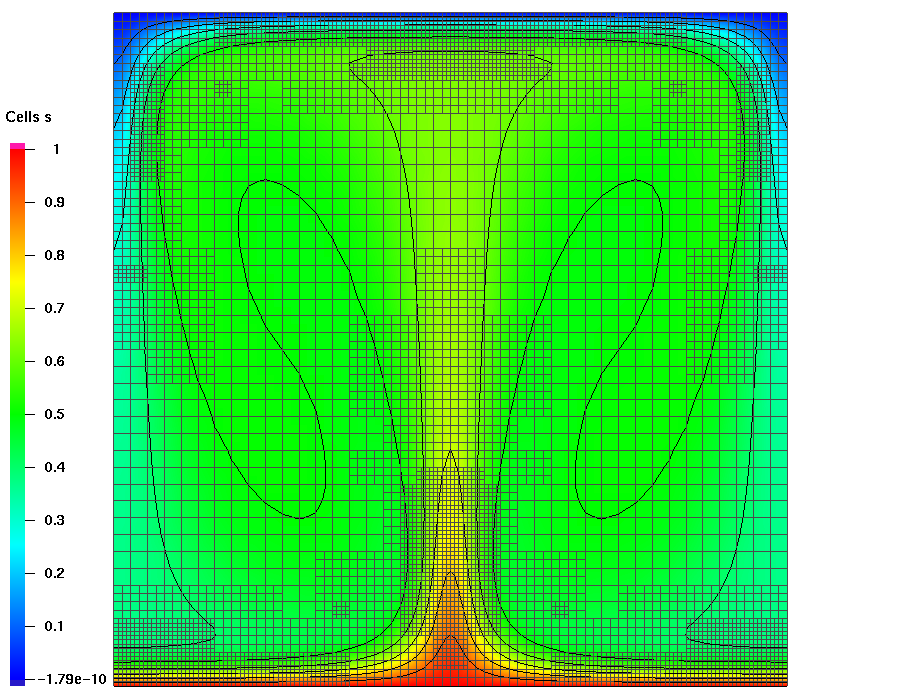
\includegraphics[width=.8\textwidth]{figures/biquad_amr_0003}    
  \end{center}
\end{frame}
\begin{frame}
  \frametitle{Biquadratic Adaptivity}
  \begin{center}
	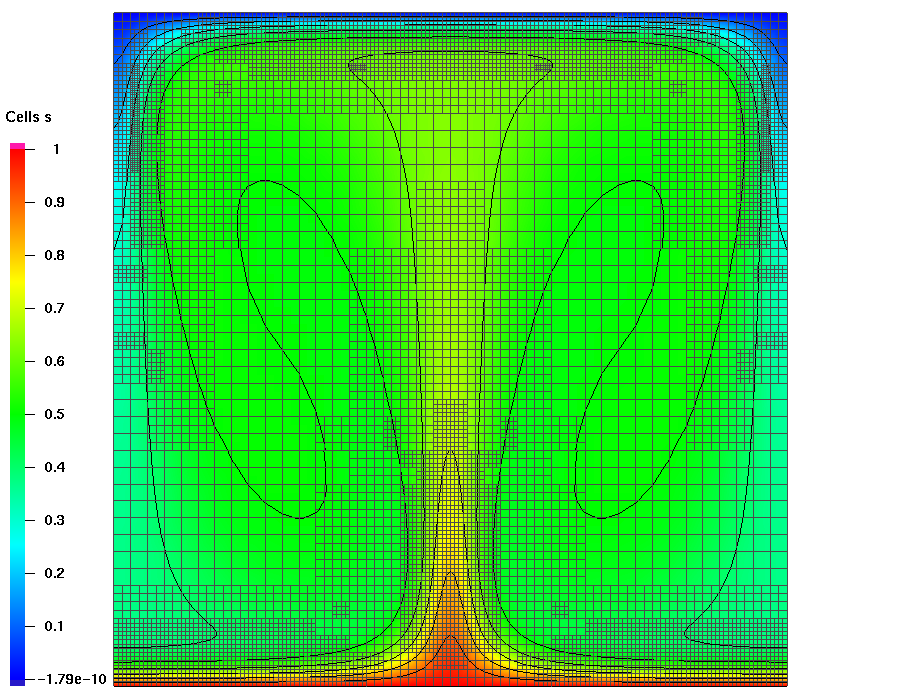
\includegraphics[width=.8\textwidth]{figures/biquad_amr_0004}    
  \end{center}
\end{frame}
\begin{frame}
  \frametitle{Biquadratic Adaptivity}
  \begin{center}
	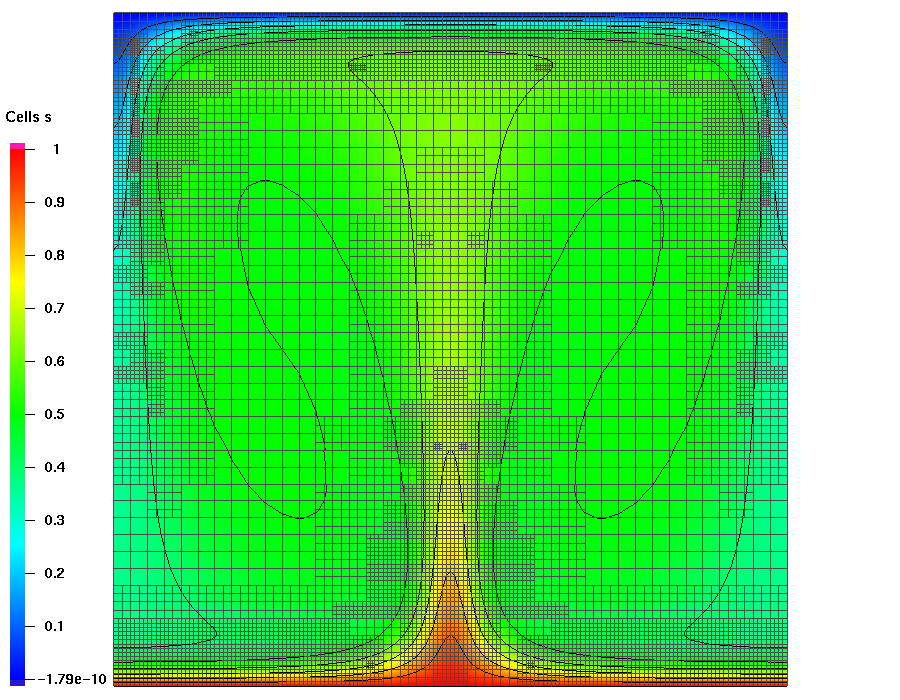
\includegraphics[width=.8\textwidth]{figures/biquad_amr_0005}    
  \end{center}
\end{frame}
\begin{frame}
  \frametitle{Biquadratic Adaptivity}
  \begin{center}
	\includegraphics[width=.9\textwidth]{figures/biquad_adapt_vs_unif_thermal}    
  \end{center}
\end{frame}
\begin{frame}
  \frametitle{Biquadratic Adaptivity}
  \begin{center}
	\includegraphics[width=.9\textwidth]{figures/biquad_adapt_vs_unif_solute}    
  \end{center}
\end{frame}







\begin{frame}
  \frametitle{Future Work}
  \begin{itemize}
    \item{Improved (practical) error indicators}
    \item{Explain higher-than-expected accuracy of classical
      flux calculation for bilinear elements} 
  \end{itemize}
\end{frame}


 

\end{document}

% LocalWords:  rcl fv Nonlinearity Dupont Cochburn Wahlbin Babu ka Bilinear
% LocalWords:  Biquadratic
